\section{Evaluation plan}
\label{sec:eval}

\subsection{Preliminary Virtualization Results}

\begin{figure}[tbh]
\centering
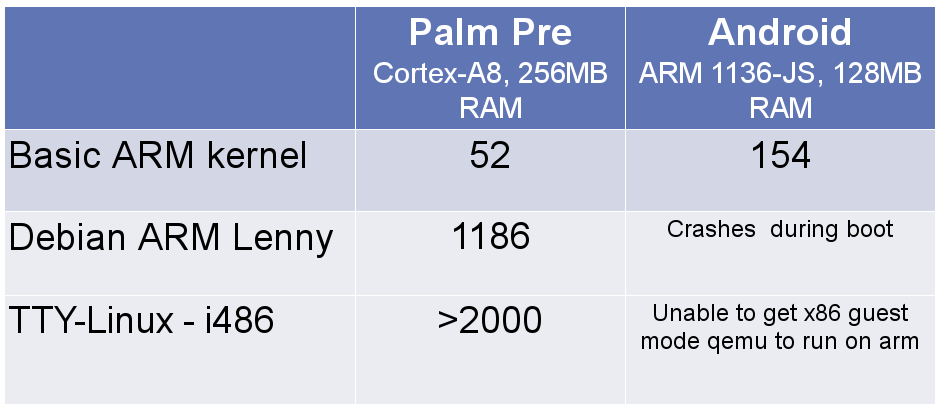
\includegraphics[width=1.0\columnwidth]{virtualization_results}
\caption{Virtualization Results: Kernel Boot time in seconds}
\label{fig:virt_results}
\end{figure}

Currently, virtualization has been tested with QEMU-based implementations running various linuxes on both the Android and the Pre \ref{fig:virt_results}.  The most successful implementation used ARM on ARM virtualization and a basic ARM kernel image provided by QEMU.  Unfortunately, even this implementation was far too slow, taking 52 seconds to boot on the Pre and 154 seconds to boot on the Android.  Additionally response times were terrible, often taking several seconds to display text input.  A Debian ARM Lenny image took over 15 minutes to boot on the Pre and crashed on the Android during boot.  X86 on ARM was also tested, with a TTY-Linux image; however, this was the slowest by far, taking over half an hour to boot on the Pre.  On the Android, x86 guest mode QEMU would not even run.

\subsection{X-Server numbers}

An important part of our system is the X server to visualize and interact with the applications.  While our current design is somewhat limited in that it has too many layers of abstractions (using SDL as the backend), we've taken efforts to make the server run faster, which resulted in a much better user experience.  The biggest  performance improvement was moving from basic SDL to SDL-GLESv2 which improved the "feel" of X and the applications inside of it noticeably.  To try to capture this speed improvement we ran x11perf, which helps quantify the performance improvements.  As shown in Figure \ref{fig:x_results}, there was noticeable improvements in a number of tests.
These tests we run from a Debian chroot, using localhost communication (not domain sockets) with the server, on the Palm Pre.  The tests were arbitrarily selected, with an attempt at finding representative ones.  These numbers should only be taken as illustrating the general performance improvements, not as an accurate measure of what real applications will be like.
\begin{figure}[tbh]
\centering
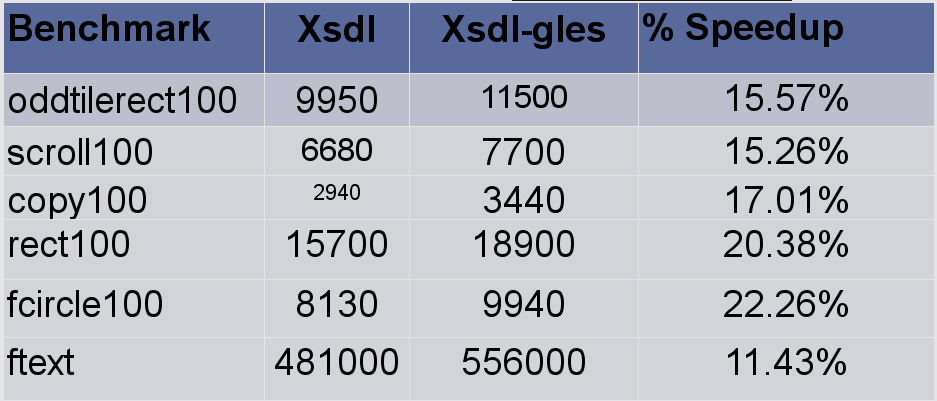
\includegraphics[width=1.0\columnwidth]{x_results}
\caption{X server rendering with x11perf}
\label{fig:x_results}
\end{figure}
